\documentclass[thesis.tex]{subfiles}

\begin{document}

\chapter{Prerequisites}\label{chap:preq}
The following sections explain some of the underlying principles that are required to understand the later chapters in this thesis.
Readers that are familiar with the basic concepts of photorealistic and realtime rendering may skip parts of this chapter.

% What belongs here:
% - Mathematics
% - Things that I would expect the reader to know if this would be a paper
% - What constraints are just there
% What does not belong here:
% - References to work that is directly related to the topic

\section{Theoretical Foundation} \label{sec:preq:theo}
This section explains some of the fundamentals of physically based rendering.
We will only discuss a few basics which are helpful for a good understanding of this thesis.
For more detailed explanations the reader is referred to the book \emph{Physically Based Rendering, From Theory to Implementation} by Pharr and Humphreys \cite{bib:pbrt}.

\subsection{Physical Foundation}
Light is generally an electromagnetic wave which originates at a light source and is bounced of or absorbed by the surfaces it hits.
As such, there are several complicated physical properties like diffraction,interference and quantization effects (due to the particle properties of electromagnetic waves) which are usually ignored for rendering, as they play most of the time a minor role.
Each light particle (= photon) has a certain wavelength which is responsible for the perceived color.
We are only interested in the visible part of the spectrum which ranges from about $380nm$ to $780nm$.
The number of photons registered by the eye defines the brightness.
\\
As the human retina has only three receptors, each with a given range of wavelength-support, it is usually sufficient to perform all calculations using only the three basic color stimuli red, green and blue \cite{bib:colorscience}.
However, as recently pointed out by Meng et al. \cite{bib:spectrumrendering} there are several problems that might lead to color shifts and violation of energy conservation. \todo{recheck when I heared that talk (upcoming EGSR)}

\subsection{Radiometric Quantities}
There are several basic quantities that describe the transport and perception of light.
Several of them depends on a \emph{solid angle}, the 3D equivalent of a 2D arc length.
The solid angle subtended by an object is computed by the projected area on the unit sphere in a given point.
Solid angles are measured in steradians $sr$.
A solid angle representing the entire unit sphere, has $4\pi\,sr$.
As common, we use the symbol $\omega$ both for the solid angle itself and the normalized directions of a differential solid angles when integrating over (a part of) a sphere.
For example, an integration of a direction dependent function $f(\mathbf{x})$ over all directions in a hemisphere is expressed as:
\begin{equation}
\int_{2\pi\,sr} f(\omega) \, \mathrm{d}\omega
\end{equation} 
$\mathrm{d}\omega$ denotes the differential steradian, while $\omega$ alone is a single direction on the unit hemisphere.

% % % % % % % % % % % % % % % % % % % % % % % % % % % % % % % % % % % % % % % % % % % % % % % %
\begin{figure}[h]
\centering
\begin{subfigure}[b]{0.45\textwidth}
\centering
\includepdftex{flux}
\caption{Flux $\phi$, light emittance per second.}
\label{fig:flux}
\end{subfigure}
\begin{subfigure}[b]{0.45\textwidth}
\centering
\includepdftex{intensity}
\caption{Intensity $I = \frac{\mathrm{d}\phi}{\mathrm{d}\omega}$}
\label{fig:intensity}
\end{subfigure}

\vspace{10pt}

\begin{subfigure}[b]{0.45\textwidth}
\centering
\includepdftex{irradiance}
\caption{Irradiance $E = \frac{\mathrm{d}\phi_{in}}{\mathrm{d}A}$}
\label{fig:irradiance}
\end{subfigure}
\begin{subfigure}[b]{0.45\textwidth}
\centering
\includepdftex{radiance}
\caption{Radiance $L = \frac{\mathrm{d}\phi}{\mathrm{d}\omega \cdot \mathrm{d}A^\perp }$}
\label{fig:radiance}
\end{subfigure}
\caption{Sketches visualizing different radiometric quantities.}
\end{figure}
% % % % % % % % % % % % % % % % % % % % % % % % % % % % % % % % % % % % % % % % % % % % % % % %

\emph{Radiant flux} $\phi$ describes the energetic output of a light source (see \autoref{fig:flux}).
It measures how much energy a light source emits over time and is thus given in watts.
\\
\emph{Intensity} $I$ gives how much flux $\phi$ per solid angle $\omega$ is emitted in a certain direction (see \autoref{fig:intensity}).
\begin{equation}
I = \frac{\mathrm{d}\phi}{\mathrm{d}\omega}
\end{equation}
It is especially useful to describe in which direction light sources emit more or less light.
\\
Irradiance $E$ determines how much light (incoming flux $phi_{in}$) per area $A$ a surface receives (see \autoref{fig:irradiance}).
\begin{equation}
E = \frac{\mathrm{d}\phi_{in}}{\mathrm{d}A}
\end{equation}
The opposite, how much light per area is leaving a surface, is also called radiant exitance of radiosity.
However, as in many other works, we will use the term for both incident and exitant light.
\\
The last and most important quantity is \emph{radiance} $L$ since it is the which is "visible" as it corresponds to the seen brightness (see \autoref{fig:radiance}).
It is defined as emitted flux $\phi$ per solid angle $\omega$ per projected emitter area $A^\perp$ in respect to a certain detector.
\begin{equation}
L = \frac{\mathrm{d}\phi}{\mathrm{d}\omega \cdot \mathrm{d}A^\perp }
\end{equation}
The projected ("seen") differential area $\mathrm{d}A^\perp$ is depended of the angle $\theta$ between emitter surface and detector direction:
\begin{equation}
\mathrm{d}A^\perp = \mathrm{d}A \cdot \cos\theta
\end{equation}

%$\phi$ & \textbf{Radiant Flux}, light power\\
%$I$ & \textbf{Radiant Intensity}, flux density per solid angle\\
%$E$ & \textbf{Irradiance}, flux density per area\\
%$L$ & \textbf{Radiance}, flux density per area per solid angle\\

\subsection{Basic Relations and Common Types of Light Sources}
A point light is an emitter without any extent, radiating in all directions with the intensity $I$.
The irradiance in respect to such a light source declines with the square of the distance $d$ as the area "seen" by the source declines quadratically.
Additionally, the "seen" area is depended on the angle $theta$ between the light direction and the surface normal.
The resulting formula is known as photometric distance law.
\begin{equation}
E = \frac{I \cdot \cos\theta}{d^2}
\end{equation}

Another reoccurring type of light source is the spot light.
Generally, a spot light is a point light with a limited region of intensities bigger than zero.
In this thesis we define the intensity of a spot light with an opening angle of $\alpha$ that points in the direction $\mathrm{l}$ depending on as following:
\begin{equation}
I(\mathrm{d}) = \Big(\frac{(\mathrm{l} \cdot \mathrm{d}) - \cos\alpha }{1-\cos\alpha}\Big)^+ \cdot I_0
\end{equation}
\todo{how we define our spot lights is not really a basic, but it fits so nicely in here?}

A Lambert emitter is that appears equally bright from every direction.
That means that the radiance is independent of the angle under which the emitter is seen.
This results in a cosine falloff of the intensity of such an emitter:
\begin{equation}
I(\theta) = (\cos\theta)^+ \cdot I_0
\end{equation}

\subsection{Rendering Equation}
% % % % % % % % % % % % % % % % % % % % % % % % % % % % % % % % % % % % % % % % % % % % % % % %
\begin{figure}[h]
\centering
\includepdftex{renderingequation}
\caption{Schematic sketch of the rendering equation. The seen radiance $L_o(\mathrm{x}, \omega_o)$ depends on the incoming radiance $L_i(\mathrm{x}, \omega_o)$ for all directions on the hemisphere.}
\label{fig:renderingeq}
\end{figure}
% % % % % % % % % % % % % % % % % % % % % % % % % % % % % % % % % % % % % % % % % % % % % % % %
The well-known rendering equation by Kajiya \cite{bib:renderingequation} is a general description of the radiance in a given point $\mathrm{x}$ in a direction $\omega_o$:
\begin{equation}
L_o(\mathrm{x}, \omega_o) = L_e(\mathrm{x}, \omega_o) + \int_{2\pi\,sr} f_r(\mathrm{x}, \omega_i, \omega_o) \cdot L_i(\mathrm{x}, \omega_i) \cdot \cos\theta_i \, \mathrm{d}\omega_i
\end{equation}
Where $L_e$ is the self-emission and $L_i$ the incoming radiance for a given direction.
$f_r$ denotes the \emph{bidirectional reflection distribution function} (BRDF) that describes how the surface reflects light.
It will be examined more closely in the next section.
The integral sums for all directions $\omega_i$ on the hemisphere, how much light is reflected to a observer in the direction $\omega_o$.
\autoref{fig:renderingeq} visualizes the concept.
Note that the evaluation of a single $L_i$ again requires the evaluation of the entire equation.
This means that in theory the radiance at any point in any direction depends on all other points.
Approaches that try to solve or approximate this recursive property of the rendering equation are thus performing \emph{global illumination}, as opposed to \emph{local illumination} where $L_i$ only includes directly visible light sources.

One of the easiest ways of solving the rendering equation is path tracing which was presented alongside the equation.
It solves the integral via a Monte Carlo integration:
For each radiance sample multiple rays are shot into the scene.
At each intersection the emissivity of the surface is evaluated. 
The ray is reflected accordingly to the local material, using the BRDF as probability density.

There are several phenomenons which are ignored by this basic form of the rendering equation.
For example it is assumed that light travels through vacuum, i.e. no scattering or absorption within participating media occurs.

\subsection{Bidirectional Reflectance Distribution Function}\label{sec:preq:brdf}
For a given surface position, the BRDF $f_r(\omega_i, \omega_o)$ determines the ratio between the differential outgoing radiance $\mathrm{d}L$ in the direction $\omega_o$ and the differential irradiance $\mathrm{d}E$ from $\omega_i$:
\begin{equation}
f_r(\omega_i, \omega_o) = \frac{\mathrm{d}L}{\mathrm{d}E}
\end{equation}
The values of the BRDF also depend on wavelength, but as mentioned earlier we use RGB vectors instead.
Physically plausible BRDFs are always positive, are energy-preserving and give the same result if $\omega_i$ and $\omega_o$ are swapped (Helmholtz reciprocity).
The BRDF determines the color and reflectence properties of a surface.
Thus, a given configuration is often also called \emph{material}.

There are many different attempts to describe the BRDF by an analytical model.
The most basic one is the Lambert BRDF, also simply called diffuse material.
Diffuse surfaces behave like lambert emitters and distribute incoming radiance in all directions.
It is defined as:
\begin{equation}
f_r(\omega_i, \omega_o) = \frac{\rho_d}{\pi}
\end{equation}
Where $\rho_d$ is the diffuse \emph{reflectance}.
Reflectance is defined as ratio between all outgoing and all incoming light:
\begin{equation}
\rho = \frac{\phi_o}{\phi_i} = \frac{\int\limits_{2\pi\,sr} L_o(\omega_o)\cdot \cos\theta_o  \, \mathrm{d}\omega_o}{\int\limits_{2\pi\,sr} L_i(\omega_o)\cdot \cos\theta_i  \, \mathrm{d}\omega_i}
\end{equation}
It is often used in combination with a second BRDF to account for specular highlights.
Note that it is possible to combine arbitrary BRDFs as long as the combined result is still physically plausible.

In this thesis we make mainly use of the \emph{Blinn-Phong} BRDF \cite{bib:blinnphongbrdf}.
It is a very simple half-vector BRDF which delivers more plausible results than the more frequently used \emph{Phong} BRDF \cite[p.~251f]{bib:RealtimeRenderingBook}.
The half-vector $\hat{\mathbf{h}}$ is the normalized sum of direction to the light $\hat{\mathbf{d}}$ and the direction to the viewer $\hat{\mathbf{v}}$:
\begin{equation}
\hat{\mathbf{h}}_i = \frac{\hat{\mathbf{d}} + \hat{\mathbf{v}}}{||\hat{\mathbf{d}} + \hat{\mathbf{v}}||}
\end{equation}
Since the original formulation of this BRDF is not energy preserving, we use the normalization form derived by Sloan and Hoffman as described in \cite[p.~257]{bib:RealtimeRenderingBook}.
For a given surface normal $\hat{\mathbf{n}}$ and the \emph{half-vector} $\hat{\mathbf{h}}$ it is defined as:
\begin{equation}
f_r(\hat{\mathbf{n}}, \hat{\mathbf{h}}) = \rho_s \cdot \frac{\gamma + 8}{8\pi} \cdot ((\hat{\mathbf{n}} \cdot \hat{\mathbf{h}})^+)^\gamma
\end{equation}
Where $\rho_s$ is the specular reflectance (also called specular color) and $\gamma$ the specular exponent which steers the sharpness of the highlight.
Both may vary with the position on a surface.

\section{Realtime Rendering}
This section gives an overview over a few important aspects of realtime rendering.
However, it is assumed that the reader is already familiar with the most basic concepts like (camera-)transformations, (triangle) geometry setup, texture/normal mapping, filtering and mip-mapping.
Informations about these topics can be found in the book \emph{Real-Time Rendering} by Akenine-M\"{o}ller et al. \cite{bib:RealtimeRenderingBook}. %, on which parts of this section are based.
\todo{currently there is only a bit on lighting, nothing more. introduction and title does not fit!}

\subsection{Realtime Direct Lighting}
While global illumination as expressed by the rendering equation is currently very difficult to achieve, different local illumination approaches have been used successfully in productive real-time rendering for many years.

\subsubsection{Shadow Mapping}
Depending on the definition, direct lighting may already no longer dubbed as local illumination since it requires for to determine the direct visibility of all light sources. 
Visibility checks in general are a "global problem" since it is necessary to take the entire scene between light emitter and receiver into account.
Especially for non-dimensionless light sources like area or environment lights (light from the entire sky) direct visibility determination is already a difficult problem.

The most popular technique for direct shadows from dimensionless light sources is \emph{shadow mapping} \cite{bib:shadowmapping} since it maps very well today's graphics hardware.
A shadow map is a texture containing depth values rendered with the view of a corresponding light source.
When shading an object, the distance to the light source is now compared with its depth value stored in the shadow map.
If the stored value is smaller, the pixel lies in the shadow, otherwise not.

% % % % % % % % % % % % % % % % % % % % % % % % % % % % % % % % % % % % % % % % % % % % % % % %
\begin{figure}[h]
\centering
\subcaptionbox{Self-shadow aliasing caused by texels that are both bellow and above the surface. \label{fig:shadowacne}}{
	\begin{subfigure}[b]{0.45\textwidth}
		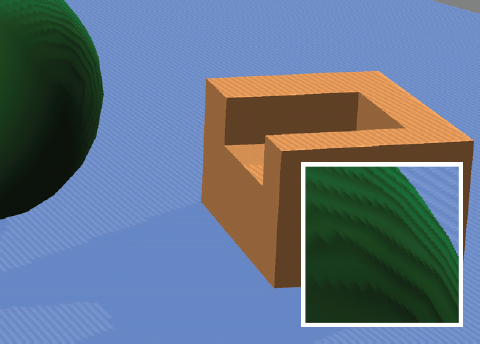
\includegraphics[width=\textwidth]{shadow/shadowacne_rtr}
   	\end{subfigure}
   	~
 	\begin{subfigure}[b]{0.45\textwidth}
	 	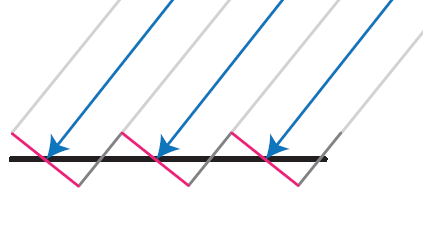
\includegraphics[width=\textwidth]{shadow/shadowacne_sketch_rtr}
 	\end{subfigure}
}
\\
\subcaptionbox{Bias fixes above issue, but now the object seems to float. \label{fig:peterpanning}}{
	\begin{subfigure}[b]{0.45\textwidth}
		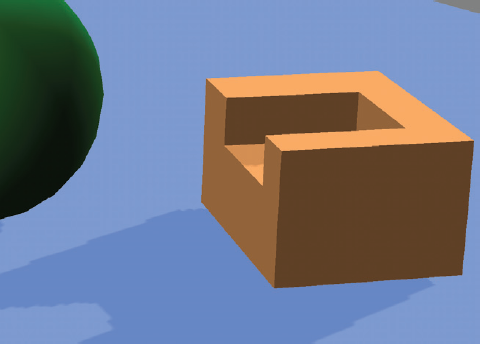
\includegraphics[width=\textwidth]{shadow/peterpanning_rtr}
   	\end{subfigure}
   	~
 	\begin{subfigure}[b]{0.45\textwidth}
	 	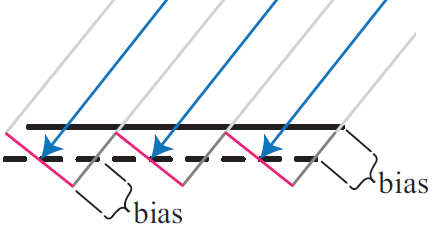
\includegraphics[width=\textwidth]{shadow/peterpanning_sketch_rtr}
 	\end{subfigure}
}
\caption{\cite[p.351]{bib:RealtimeRenderingBook} Shadow map samples surface, shown by blue arrows. The red line shows the distance that the shadow map saves.}
\end{figure}
% % % % % % % % % % % % % % % % % % % % % % % % % % % % % % % % % % % % % % % % % % % % % % % %
There are various extensions to shadow mapping that try to improve the sampling quality or simulate non-dimensionless light sources.
Shadow mapping is very prone to artifacts like self-shadow aliasing, also known as shadow acne.
Surfaces are sometimes incorrectly considered shadowing themselves since point samples from the shadow map are used to represent an area's depth, see \autoref{fig:shadowacne}.
The problem can be overcome by adding a bias to the depth values.
This however, effectively moves the surface from the light which again leads to another artifact known as "Peter Panning":
For a too large bias, objects are disconnected from their shadows which leads to a floating appearance, see \autoref{fig:peterpanning}.
\\
To alleviate this issue, Holbert \cite{bib:normaloffsetshadowmapping} introduced a normal dependent offsetting approach:
Positions are offset not just in direction of the shadow projection, but in the direction of the surface normal depending on the angle to the light direction.
This allows much lower bias values without self-shadow aliasing.

In our implementation we use shadow maps combined with normal offset mapping to determine the direct visibility of spot lights. \todo{if there were light types added, note here (and earlier to describe the type?)}

\subsubsection{Deferred Shading}
In classic "forward rendering" the rendering and shading of objects is coupled.
To be able to use multiple lights (for direct lighting), shading procedures either involve loops over all light sources or rendering all objects multiple times using only one light each time (multipass lighting).

Deferred shading decouples object rendering and pixel shading by saving all information needed for shading in the so called G-buffer. \todo{gbuffer image!}
This buffer usually saves for each pixel a depth (which can be used to reconstruct the world position), normal and material properties.
Afterwards used to compute dynamic illumination in a screen-space pass without re-rendering the scene geometry itself for these passes.
The approach scales very well with many lights and can reduce the general complexity of a renderer considerably.
Overdraw occurs only during the G-buffer creation which makes expensive BRDF calculations more viable.
The main drawbacks of deferred shading include difficulties with multisampling-antialiasing and the need to handle transparent objects separately.

\section{Modern GPU Pipeline and Capabilities}
In this section several concepts of modern graphics hardware are introduced.
These are not only necessary to understand implementation details, but also some of the decisions about on the design of the presented algorithm.
As we rely on the open graphics API OpenGL 4.5, we make use of terms and names as they are defined in the OpenGL (core) specification \cite{bib:openglspec}.
Note that these are sometimes different from those used by the hardware vendors and other APIs.

%As of this writing, OpenGL 4.5 is the most recent
%While we are aware that the API abstraction layer often does not reflect the underlying hardware, throughout this thesis we usually operate only on 

\subsection{Rendering Pipeline Overview}
% % % % % % % % % % % % % % % % % % % % % % % % % % % % % % % % % % % % % % % % % % % % % % % %
\begin{figure}[h]
\centering
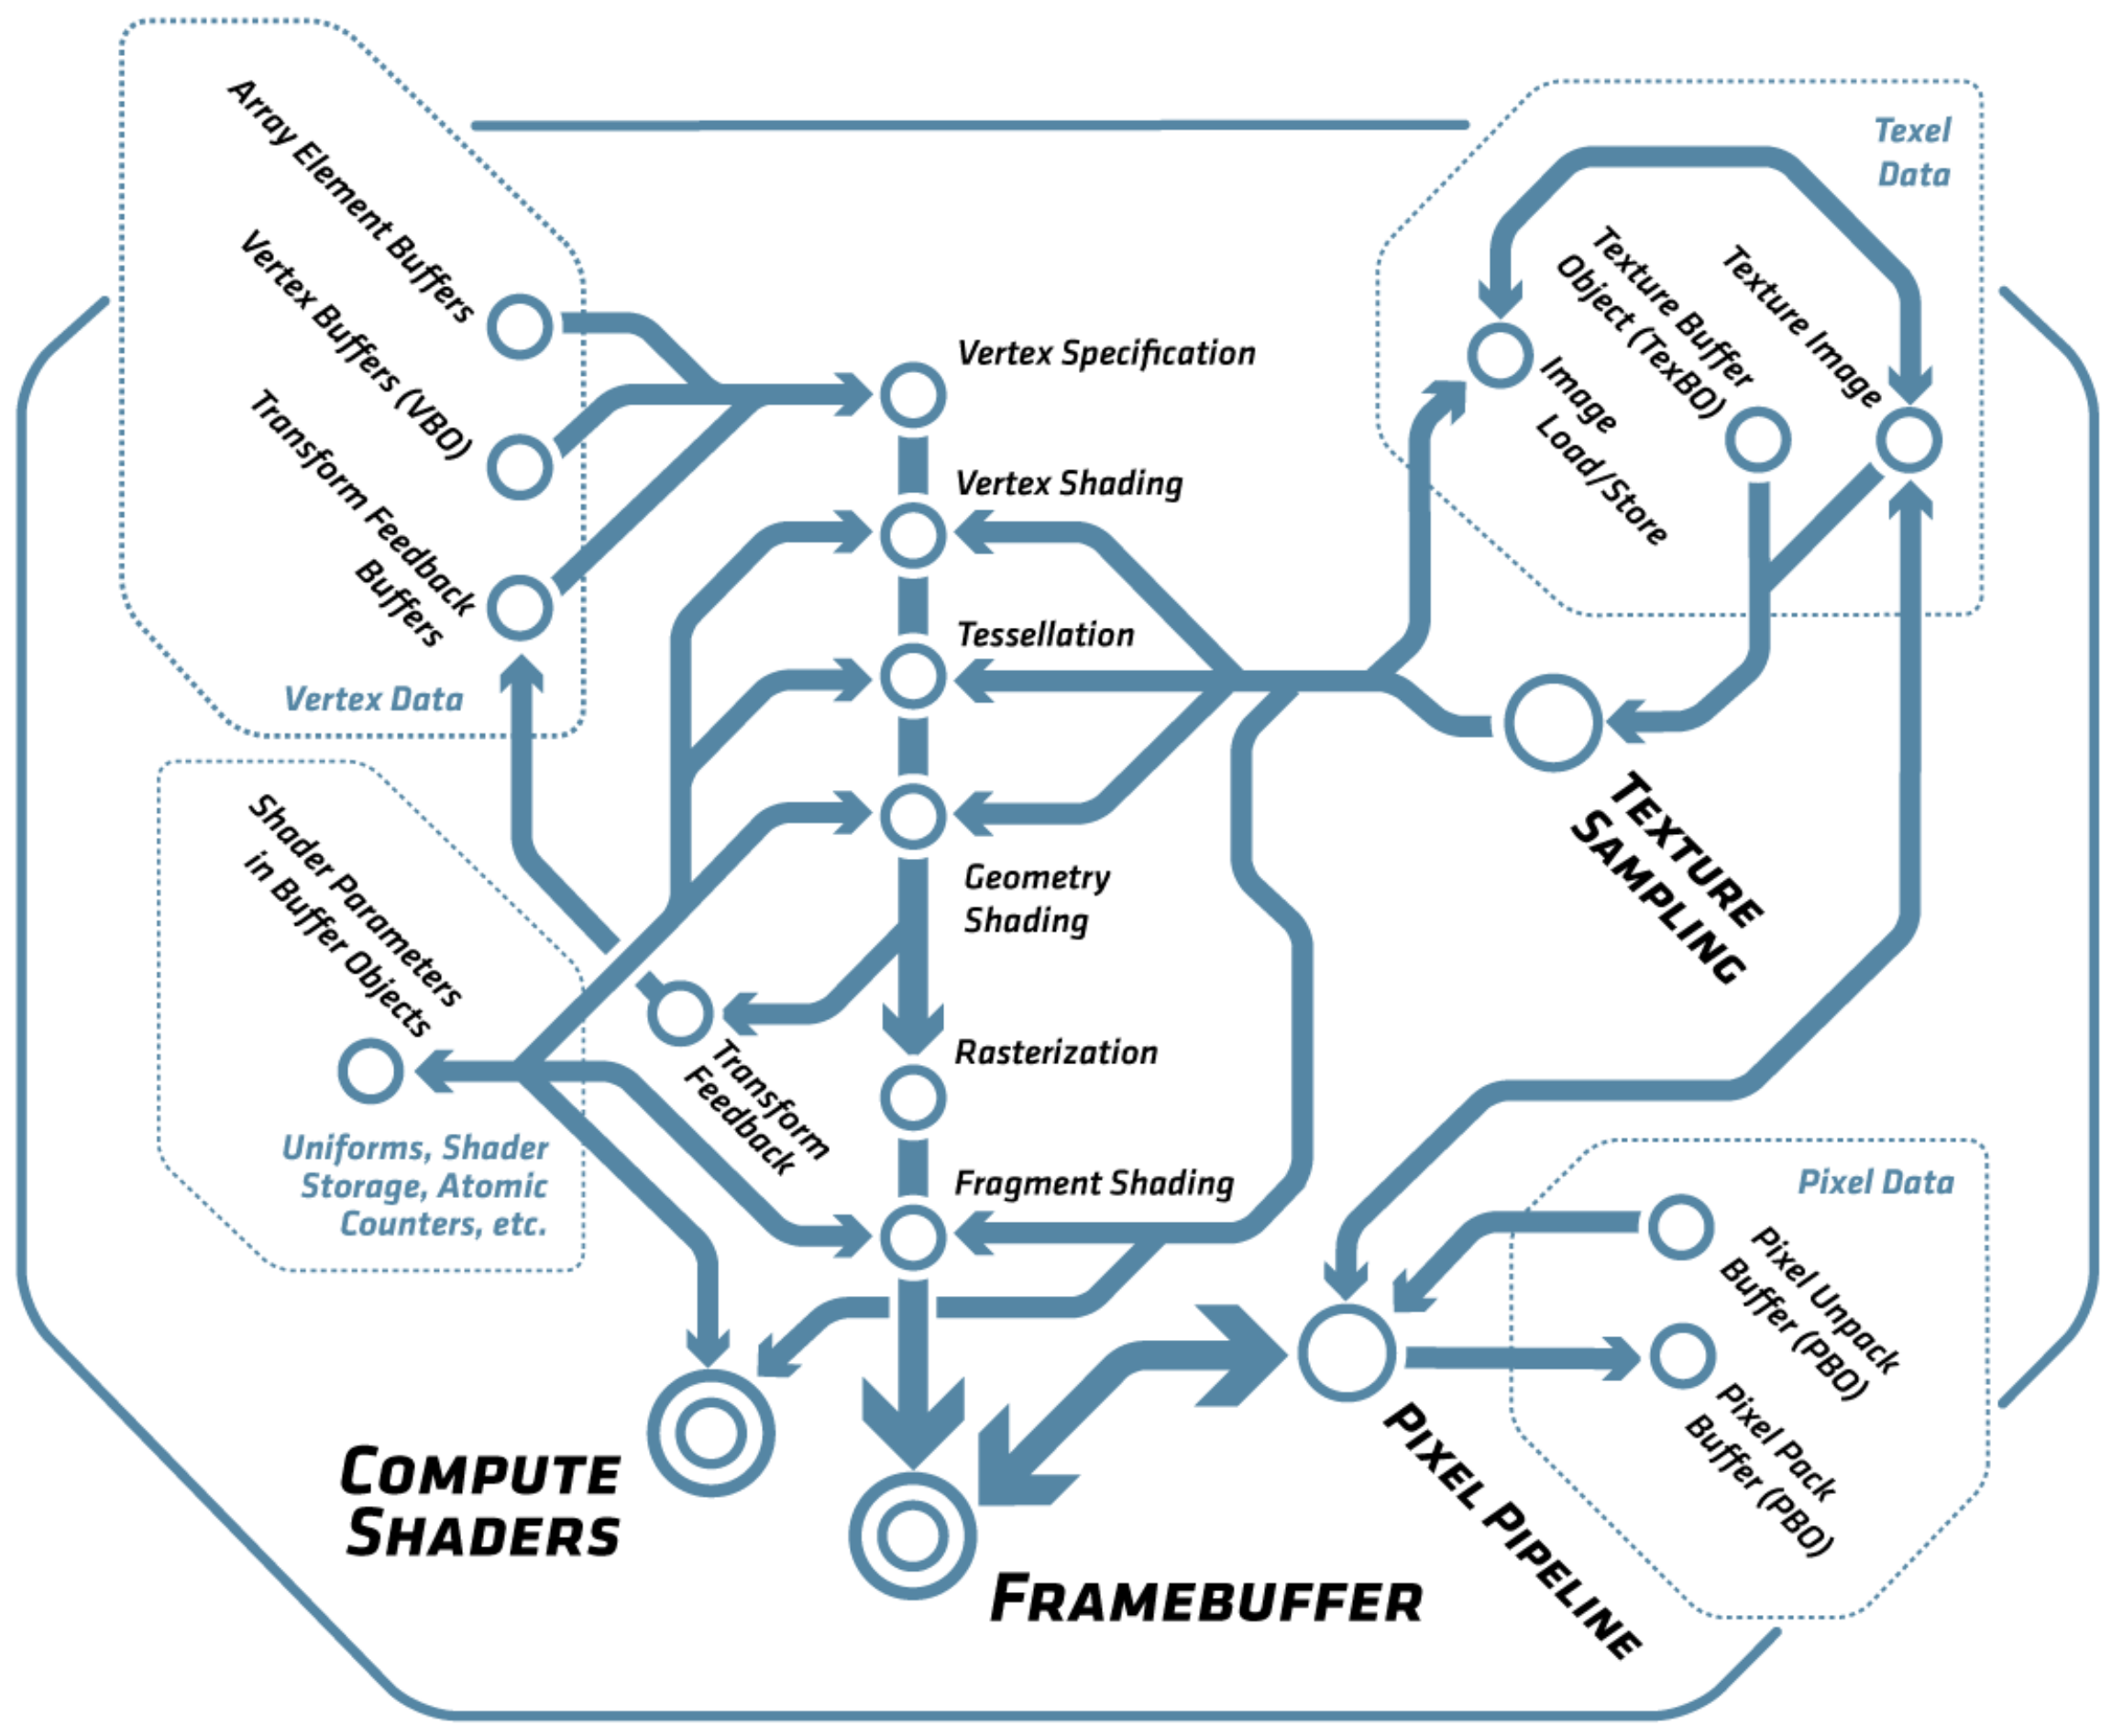
\includegraphics[width=\textwidth]{opengl45pipeline}
\caption{\cite{bib:openglspec} Official OpenGL 4.5 pipeline overview.}
\label{fig:openglpipe}
\end{figure}
% % % % % % % % % % % % % % % % % % % % % % % % % % % % % % % % % % % % % % % % % % % % % % % %
\autoref{fig:openglpipe} gives a coarse overview over the modern OpenGL pipeline.
The four dashed boxes visualized different types of memory or rather ways to access memory.
As memory accesses play a major role, \autoref{sec:preq:memory} goes into further detail.
With the exception of compute shaders, all major programmable stages are on the arrow starting at "Vertex Specification" and ending at "Framebuffer".
The underlying processing is what is usually called the rendering pipeline, which is traversed by the GPU on each issued draw call.
Compute shader are outside of this pipeline and handled in the next section.
Within the rendering pipeline there are several \emph{shader} stages: Vertex shader, two shaders for tessellation, geometry and fragment shader.
Generally, shaders are small programs that issued in parallel that take data from the previous pipeline step and output data to the next, usually under the use of globally available resources.
Shaders in OpenGL are written in a specific language called GLSL which is compiled by the graphics driver to run on the GPU.
All shaders in the pipeline need to provide a specific set of outputs they and have access to several guaranteed inputs.
However, it is possible to transfer almost arbitrary additional data between the stages.
How these data is processed depends on the concrete stage and its configuration.

\subsubsection{Vertex Processing}
Vertex shader fetch data provided by previously specified vertex buffer.
The shader is invoked for each vertex.
An invocation has only access to the vertex it is assigned to.
A vertex shader must at least output a position which is later used during the rasterization stage.
This stage is mostly used for all sort of vertex transformations.

Afterwards, the tessellation stage is executed optionally.
It is skipped here, as we do not make use it in this thesis.
The following, also optional, geometry shading stage is invoked per triangle.
It is able to generate new geometry on-the-fly.
Before the advance of compute shaders, their ability to stream vertex data back to the memory (Transform Feedback) was very important for many algorithms.
Nowadays, their use is very limited as many of their former tasks can be more effectively performed by compute shaders.
In this thesis we only need them to implement a realtime voxelization algorithm (see \autoref{sec:impl:voxelization}).


%For several hardware implementation reasons, geometry generation proved to be rather slow on mot 

\subsubsection{Pixel Processing}
The rasterization stages generates pixels from the processed geometry and invokes the fragment shader for each of them.
Depending on various multisampling parameters, the fragment shader might be invoked for fragments of pixels, thus the name.
The task of the fragment is to output a color which will be written (or blended into) one or more framebuffers (also called render-target).
As long as not configured otherwise, the fragment shader is provided with perspective correct interpolated output from the last active stage preceding the rasterizer.
If a depth buffer is used, the rasterizer will perform depth tests to fulfill a previously defined condition, usually to assure that nearer triangles are not overdrawn by more distant ones.

\subsection{Compute Shader}
gpgpu stuff...
Scheme, what can it do...
Mention Occupancy!
Shared mem in next chapter

\subsection{Memory} \label{sec:preq:memory}
transfer costs, type of access - ssbo, ubo, texture, image, shader: shared, register\\
almost no restrictions (few exceptions like: cant bind texture as buffer, but vice versa)



\section{Spherical Harmonics}\label{sec:preq:sh}
Spherical Harmonics (SH) are a set of orthonormal basis functions, analogous to the Fourier transform's basis functions, but defined on the surface of a sphere.
They are often used in computer graphics to approximate spherical functions like visibility, lighting or reflectance. Similarly, they will later be used in \autoref{sec:impl:diffuse} to describe the total irradiance for a given normal.

More detailed explanations can be found for example in \cite{bib:grittysh, bib:stupidsh} on which this summary is based.

\subsection{Definition} \label{chap:sh:def}
\begin{figure}[h]
	\centering
	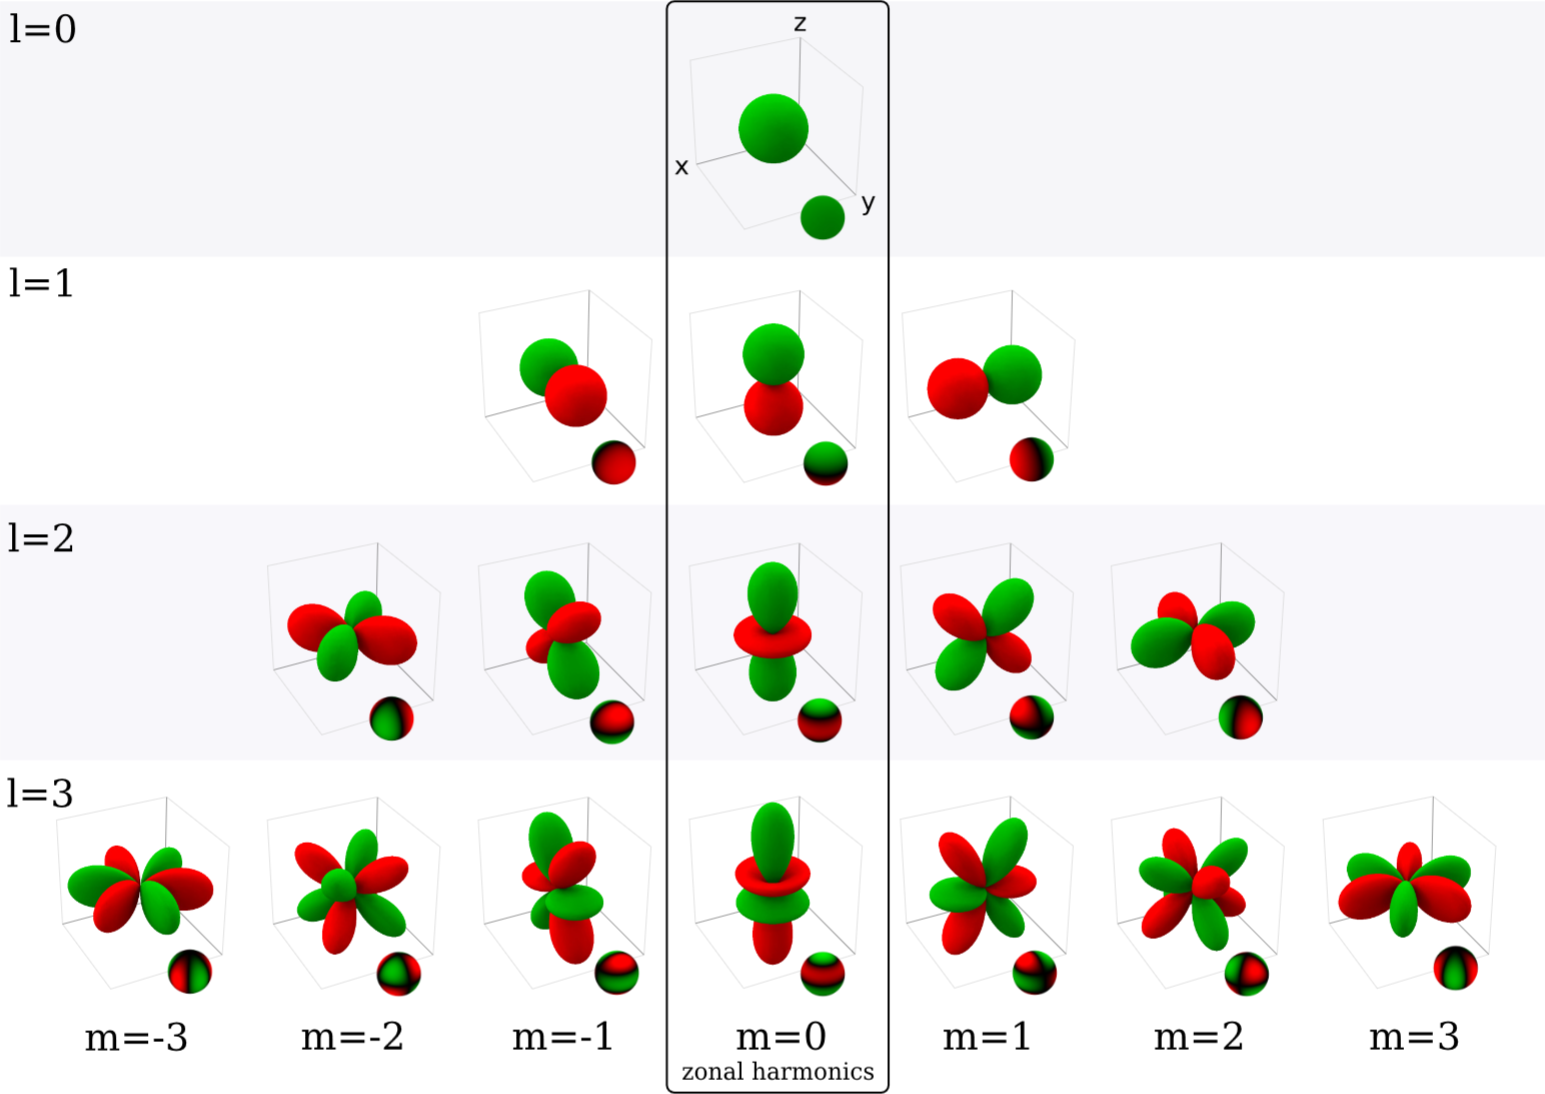
\includegraphics[width=\textwidth]{sh}
	\caption{\cite{bib:grittysph} The first three SH bands plotted as unsigned spherical functions by distance from the origin unit sphere. Green are positive values, red are negative ones.}
	\label{fig:shvisualization}
\end{figure}
\todo{Better image quality!}
The SH functions in general are defined on imaginary numbers, but for use in computer graphics usually only real-number Spherical Harmonics are relevant.

$y^m_l(\theta, \varphi)$ represents a Spherical Harmonic function.
The angles $\theta$ and $\varphi$ give a point on the unit hemisphere.
To convert from spherical to cartesian coordinates we use the following conversion:
\begin{equation} \label{equ:postoangle}
(\sin\theta\cos\varphi, \sin\theta\sin\varphi, \cos\theta) \rightarrow (x,y,z)
\end{equation}
The index $l$ represents the Spherical Harmonic \emph{band}.
Each band consists of polynomials of the degree $l$ (zero is a constant function, 1 is linear, etc.).
There are $2l+1$ functions for a given band.
Accordingly, the higher the band index $l$, the higher is the frequency of the information that is encoded in this band.
\autoref{fig:shvisualization} visualizes the first three bands.

$y^m_l(\theta, \varphi)$ is defined as:
\begin{equation}
	\begin{alignedat}{2}
		y^m_l(\theta, \varphi) &= \begin{cases}
		\sqrt{2}K^m_l \cos(m\varphi) P^m_l(\cos\theta) & m>0\\
		\sqrt{2}K^m_l \sin(-m\varphi) P^{-m}_l(\cos\theta) & m<0\\
		K^0_l P^0_l(\cos\theta) & m=0.\end{cases}
	\end{alignedat}
\end{equation}
Where $P^m_l(x)$ are the associated \emph{Legendre} polynomials and $K^m_l$ are normalization constants defined as:
\begin{equation}
	K^m_l = \sqrt{\frac{(2l+1)(l-|m|)!}{4\pi(l+|m|)!}}
\end{equation}

The associated Legendre polynomials are recursively defined as following:
\begin{equation}
	\begin{alignedat}{2}
		P^0_0(x) &= 1\\
		P^m_m(x) &= (1-2m)P^{m-1}_{m-1}\\
		P^m_{m+1}(x) &= x(2m+1)P^m_m\\	
		P^m_l(x) &= \frac{x(2l-1)P^m_{l-1}(x)-(l+m-1)P^m_{l-2}}{l-m}
	\end{alignedat}
\end{equation}


\subsection{Projection and Reconstruction} \label{chap:shprojectrecon}
Each spherical function $f(\theta, \varphi)$ can be represented with an infinite series of SH functions, each weighted by a SH coefficient.
To calculate a SH coefficient for a given band of a spherical function $f$, the product of $f$ and the SH function $y$ needs to be integrated:
\begin{equation} \label{eq:shprojection}
	c^m_l=\int\limits_{2\pi sr} f(\omega)y^m_l(\omega)\, \mathrm{d}\omega
\end{equation}
\todo{$2\pi sr$ integral must be introduced earlier}

By truncating the SH representation to $n$ bands, a function $f$ can be approximated:
\begin{equation}
	\widetilde{f}(s) = \sum_{l=0}^{n-l}\sum_{m=-l}^l c_l^m y_l^m(s)
\end{equation}

\subsection{Rotation and Zonal Harmonics} \label{sec:preq:zonalharmonics}
Spherical Harmonics are rotationally invariant:
If a function $g$ is a copy rotated by $R$ named $f$, then for the corresponding SH projections $\widetilde{g}$ and $\widetilde{f}$ it is true that:
\begin{equation}
	\widetilde{g}(s) = \widetilde{f}(R(s))
\end{equation}
This means that it is possible to rotate a function in its SH representation, without losing precision (other than rounding errors).

Later on this property will be very useful combined with \emph{Zonal Harmonics}.
Zonal Harmonics are SH projections of functions that have rotational symmetry around an axis.
If the axis is Z (in respect to \autoref{equ:postoangle}), then only the $c^m_0$ coefficients of the SH projection will be non-zero.\\
Rotation of such Zonal Harmonics $z_l$ to a new direction $d$ is generally much easier than arbitrary SH.
The resulting, rotated Spherical Harmonics coefficients are obtained as:
\begin{equation} \label{eq:zonalrotate}
	c_l^m = \sqrt{\frac{4\pi}{2l+1}} z_l y_l^m(d)
\end{equation}
\todo{Image of Zonal Harmonics}

\subfilebib % Makes bibliography available when compiling as subfile
\end{document}